\section{\textit{Picture Processing Unit} (PPU)}\label{sec:ppu}

La unidad de procesamiento de imágenes de la Game Boy Advance procesa la información de las secciones OAM, VRAM y RAM de paleta, mostradas en la Tabla~\ref{tab:mapa}, para producir una imagen que el jugador pueda ver. En la Sección~\ref{sec:arquitectura} se detallaron los modos existentes según la PPU trata lo datos. Diferenciamos tres: \textbf{\textit{Sprites}}, \textbf{\textit{Bitmaps}} y \textbf{Fondos} \cite{bib:gba_manual}. En las próximas secciones se comentarán cada uno de estos modos y sus diferentes variaciones y configuraciones.

Sin embargo, antes de indagar en cada uno de los modos hace falta entender conceptos como los \textit{tiles}. Estos son necesarios al hablar de los modos de \textit{sprites} y \textit{fondos}, la forma en la que el programador posiciona los píxeles y objetos en pantalla, y el formato utilizado para representar colores en la consola. Todos son conceptos indispensables para cualquiera de los modos que ofrece la consola de Nintendo.

Los \textit{tiles} denotan unas pequeñas imágenes (normalmente cuadradas) que sirven como base para crear escenarios y personajes. Para facilitar la comprensión de este proceso, se muestra a continuación un ejemplo en \textit{Tiled} (véase sección~\ref{sec:herr_graficas}) donde se crea un escenario (o fondo) a partir de imágenes base de un tamaño de 32 x 32 píxeles. Al conjunto de imágenes base (\textit{tiles}) se le denomina \textit{tileset}. En la Figura~\ref{fig:tiled_demo_1} se muestra un \textit{tileset} en el que se puede distinguir cada unidad por la separación que hace \textit{Tiled}.

A partir de este conjunto de imágenes base, se crea la imagen final. El proceso se puede observar en las Figuras~\ref{fig:tiled_demo_2} y~\ref{fig:tiled_demo_3}.

\begin{figure}[h]
	\centering
	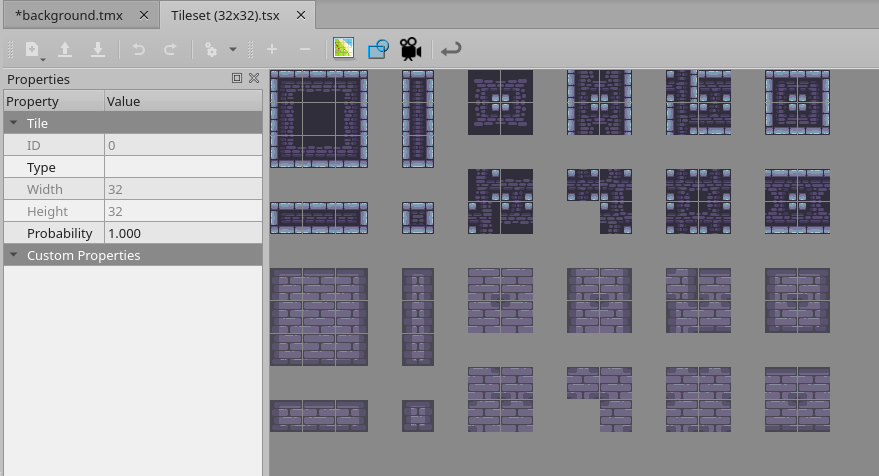
\includegraphics[width=.7\textwidth]{capitulos/capitulo3/tiled_demo_1.png}
	\caption{\textit{Tileset} que se utilizará para crear el fondo.}
	\label{fig:tiled_demo_1}
\end{figure}

\begin{figure}[h]
	\centering
	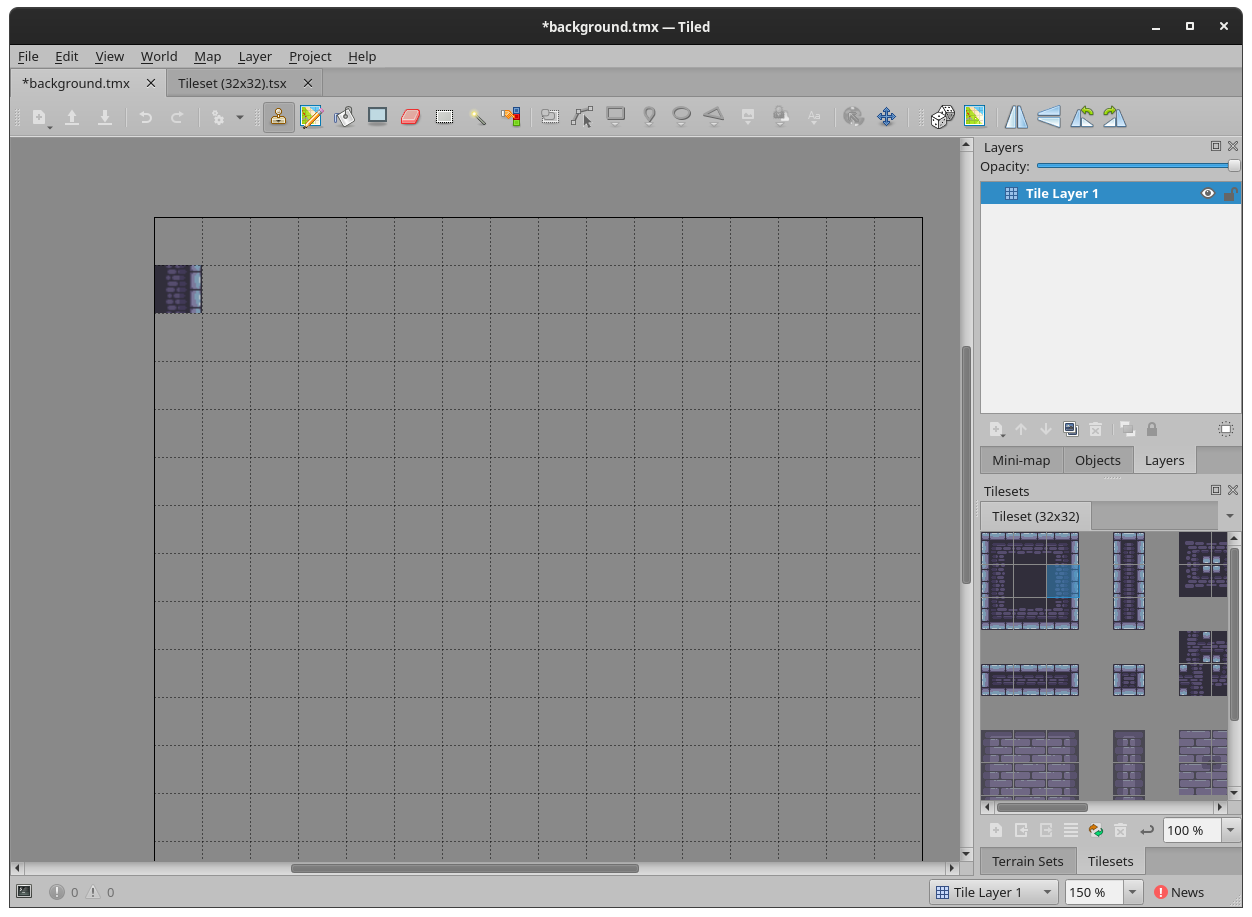
\includegraphics[width=.6\textwidth]{capitulos/capitulo3/tiled_demo_2.png}
	\caption{Relleno del canvas a partir de \textit{tiles}.}
	\label{fig:tiled_demo_2}
\end{figure}

\begin{figure}[h]
	\centering
	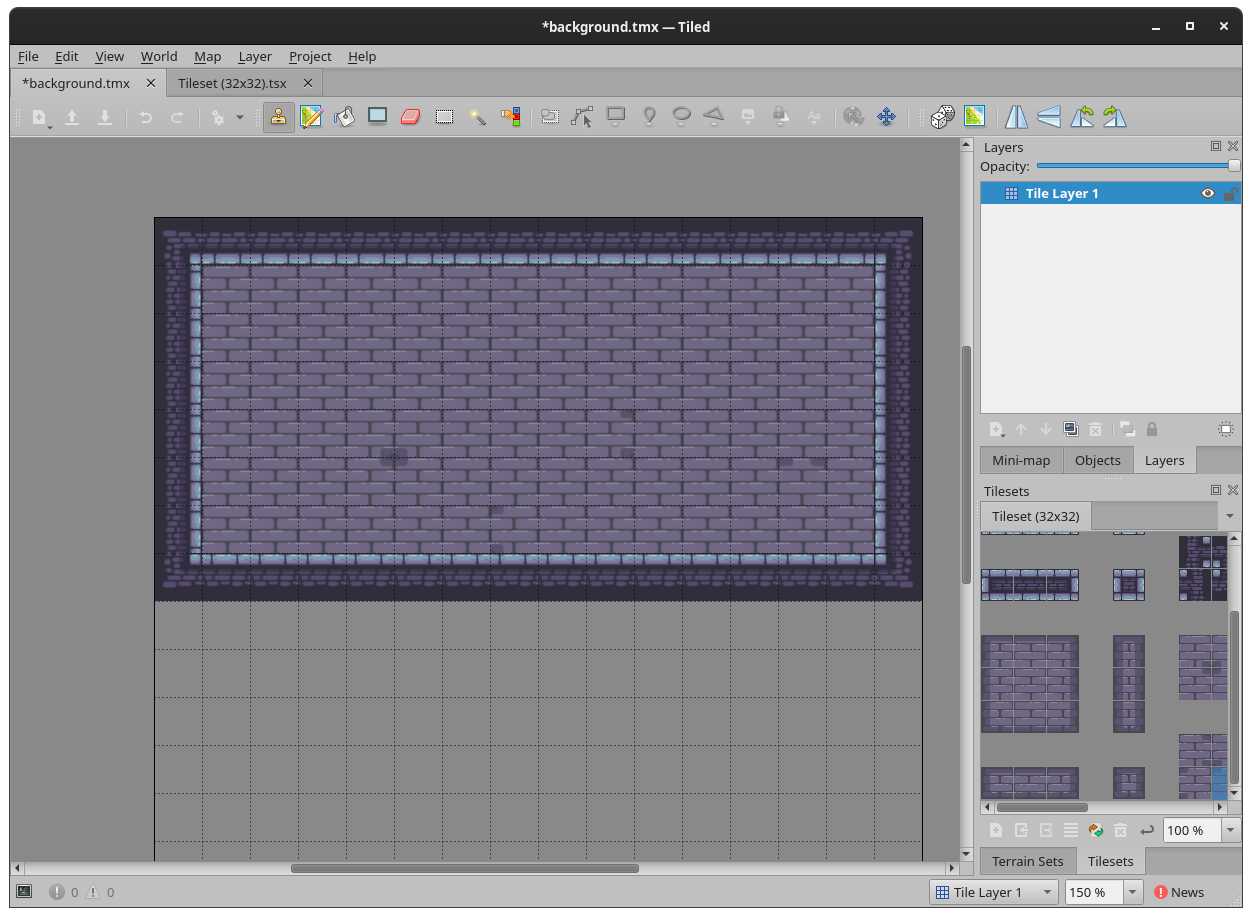
\includegraphics[width=.6\textwidth]{capitulos/capitulo3/tiled_demo_3.png}
	\caption{Creación de un fondo a partir del \textit{tileset}.}
	\label{fig:tiled_demo_3}
\end{figure}
\FloatBarrier

Esta metodología facilita la reutilización de recursos. No obstante, utilizar esta técnica requiere crear una tabla de índices adicional (o mapa) para poder especificar qué \textit{tile} se está utilizando \cite{bib:tonc}.

La reutilización se hace evidente si se consulta de nuevo la Figura~\ref{fig:tiled_demo_3} y se intenta identificar el número total de \textit{tiles} utilizados. En dicha Figura se utilizan 16 \textit{tiles} diferentes. En el caso de la Game Boy Advance este número se reduciría a 9, ya que en la tabla o mapa se puede especificar la orientación (invertir el eje horizontal o vertical) del \textit{tile}. La Figura~\ref{fig:tiled_demo_4} muestra el fondo junto con el índice de cada \textit{tile}.

\begin{figure}[h]
	\centering
	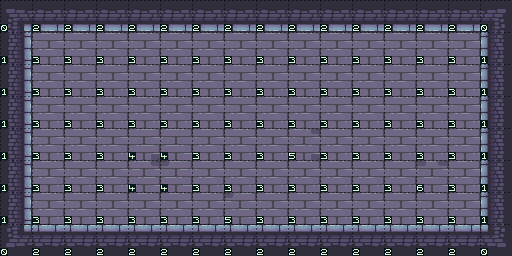
\includegraphics[width=.8\textwidth]{capitulos/capitulo3/tiled_demo_4.png}
	\caption{Distintos \textit{tiles} utilizados.}
	\label{fig:tiled_demo_4}
\end{figure}

En varias de las funciones que ofrece la \textit{PPU} es necesario especificar el posicionamiento de los \textit{tiles} a utilizar para poder renderizar la imagen correctamente. Es por esto que los \textit{tiles} se distribuyen en 32 grupos de 2048 bytes cada uno (conocidos como ``screenblocks'' en \cite{bib:tonc}). Estos grupos, a su vez, se organizan en 4 bloques todavía más abstractos de 16 KB cada uno (conocidos como ``charblocks'' en \cite{bib:tonc}). La distribución de los grupos descritos anteriormente sobre la VRAM se puede observar en la Tabla~\ref{tab:dist_charblocks}.

\begin{table}[h]
	\centering
	\begin{tabular}{| c | c | c | c | c |}
		\hline
		\textbf{Memoria} & 0x06000000 & 0x06004000 & 0x06008000 & 0x0600C000 \\ \hline
		``charblock'' & 0 & 1 & 2 & 3 \\ \hline
		``screenblock'' & \{0-7\} & \{8-15\} & \{16-23\} & \{24-31\} \\ \hline
	\end{tabular}
	\caption[Distribución de los \textit{tiles} en la VRAM.]{Distribución de los \textit{tiles} en la VRAM~\cite{bib:tonc}.}
	\label{tab:dist_charblocks}
\end{table}
\FloatBarrier{}

Para poder programar para el dispositivo, es necesario conocer también cómo trabaja la Game Boy Advance al posicionar píxeles y objetos en pantalla, además de cómo y cuándo se refresca la imagen.

Como se puede deducir de la distribución utilizada para los \textit{tiles}, la Game Boy Advance trata a la imagen como una matriz cuyas filas conforman el eje Y y las columnas el eje X. El punto de partida para los ejes, en el que su valor es 0, se posiciona en la esquina superior izquierda de la pantalla (véase la Figura~\ref{fig:y_x}).  Esto será de utilidad no solo en los modos \textit{bitmap} donde el programador manipulará la imagen a nivel de píxeles, sino también al trabajar con objetos y fondos, dado que será necesario indicar unas coordenadas para moverlos y posicionarlos.

\begin{figure}[h]
	\centering
	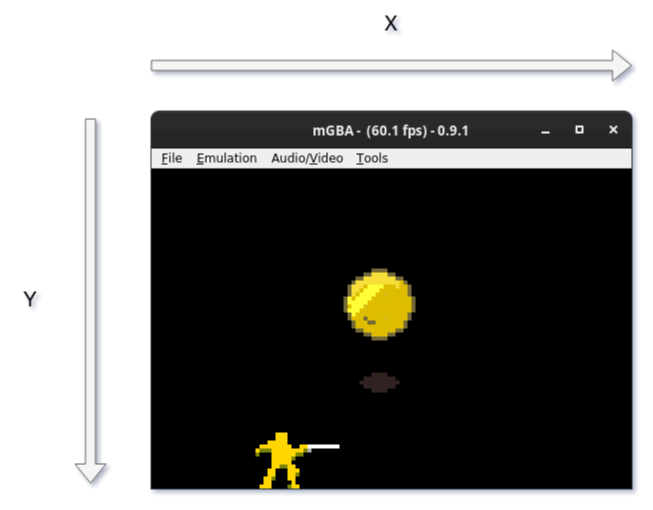
\includegraphics[width=.7\textwidth]{capitulos/capitulo3/y_x.png}
	\caption{Coordenadas de la pantalla.}
	\label{fig:y_x}
\end{figure}
\FloatBarrier

Al contrario de lo que pueda parecer, la forma en la que la pantalla de la Game Boy Advance se refresca influye en la manera en la que se programa para el dispositivo. Cada fotograma nuevo es actualizado no de ``golpe'', sino línea a línea (cada una de estas líneas recibe el nombre de \textit{scanline}). Entre cada línea refrescada existe un período llamado HBlank, y entre cada imagen refrescada existe un período llamado VBlank. Ambos ofrecen al programador un rango de tiempo en el que modificar ciertos parámetros sin distorsionar la imagen\footnote{En el caso de HBlank, esto no es del todo cierto en todos los casos dado que si se actualiza un \textit{sprite} durate HBlank es posible que se vea distorsionado.}. En total, la GBA cuenta con 228 \textit{scanlines} (el número de píxeles verticales más 68) de una longitud de 308 (el número de píxeles horizontales más 68). La Figura~\ref{fig:vblank_hblank} muestra los conceptos comentados anteriormente.

\begin{figure}[h]
	\centering
	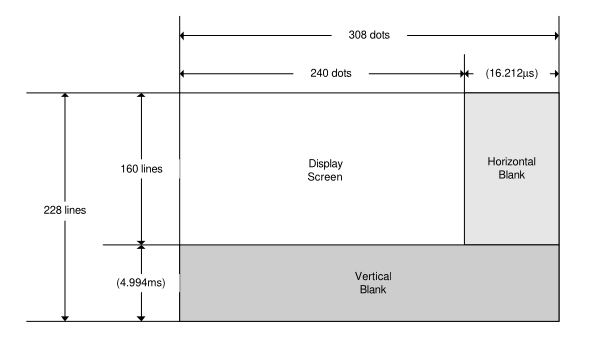
\includegraphics[width=.7\textwidth]{capitulos/capitulo3/lcd.png}
	\caption{Los períodos HBlank y VBlank en la pantalla de la GBA\@. Imagen de~\cite{bib:gba_manual}.}
	\label{fig:vblank_hblank}
\end{figure}
\FloatBarrier

Finalmente, queda mencionar que la consola utiliza un formato de 15 bits para representar colores. La distribución del rojo, verde y azul en este formato aparece representada en la Tabla~\ref{tab:15bit_color}. Como puede observarse, el bit más significativo no se usa \cite{bib:gba_manual}.

\begin{table}[h]
	\centering
	\begin{tabular}{| l | l | l | l | l | l | l | l | l | l | l | l | l | l | l | l |}
		\hline
		\o  & B & B & B & B & B & G & G & G & G & G & R & R & R & R & R \\ \hline
	\end{tabular}
	\caption{Color de 15 bits.}
	\label{tab:15bit_color}
\end{table}

Partiendo de los conceptos previos, se comentará a continuación el uso y funcionamiento de los mismos aplicados a los \textit{sprites}, fondos y \textit{bitmaps} de la Game Boy Advance.

\subsection{\textit{Sprites}}\label{sec:sprites}
La Game Boy Advance implementa a nivel de hardware un modo para manejar y mostrar personajes u objetos dentro del juego. \textit{Sprite} es el término que normalmente se utiliza para describir cualquier entidad única que se pueda mover dentro de un juego. El programador define los parámetros correspondientes y la \textit{PPU} se encargará de mostrar la imagen con los \textit{tiles} y colores que el programador haya posicionado en la VRAM y RAM de paleta, respectivamente. 

Por suerte para el programador, las tareas que se pueden considerar ``complejas'' las realiza la \textit{PPU} (por ejemplo, organizar los \textit{tiles}, tener en cuenta los bits por píxel y mostrarlos por pantalla). Aún así, tendrá que realizar los siguientes pasos para acabar mostrando el \textit{sprite} deseado:

\begin{enumerate}
	\item Separar los colores utilizados en una imagen, como un personaje o un objeto dentro del juego. Como resultado obtendremos una imagen con los índices apuntando a la paleta de colores.
	\item Dividir la imagen en bloques de 8x8, que es el tamaño base con el que trabaja la Game Boy Advance. Es en este punto donde se hace evidente la utilidad de herramientas como Grit, que automatiza la mayor parte de este proceso.
	\item Especificar las propiedades que tendrá el sprite en la OAM. Para ello, previamente, se han tenido que copiar los colores utilizados al espacio de memoria reservado para la paleta de colores y la distribución de los \textit{tiles} (los índices) a la VRAM.  Cada objeto almacenado en este espacio de memoria, que soporta hasta 128 \textit{sprites}, cuenta con tres atributos de 16 bits para definir sus propiedades.
	\item Indicar los valores que tendrán las matrices de transformación de 2x2 que se usen para rotar y escalar los \textit{sprites}. Este punto es opcional y se detallará más en profundidad en el apartado~\ref{sec:aff_obj}).
\end{enumerate}

La distribución de cada uno de estos atributos, junto con los valores de la matriz de transformación, siguen el formato expuesto en la Figura~\ref{fig:oam_dist} \cite{bib:tonc}. En dicha figura se utiliza $p$ para denotar al personaje u objeto, $Attr$ para cada uno de sus atributos y $a$ para referirse a los valores de la matriz. Es necesario recalcar que, mientras que la información de un \textit{sprite} es almacenada de forma contigua, los valores de la matriz de afinidad se encuentran dispersos, con 6 bytes de diferencia entre cada uno.

\begin{figure}[h]
	\centering
	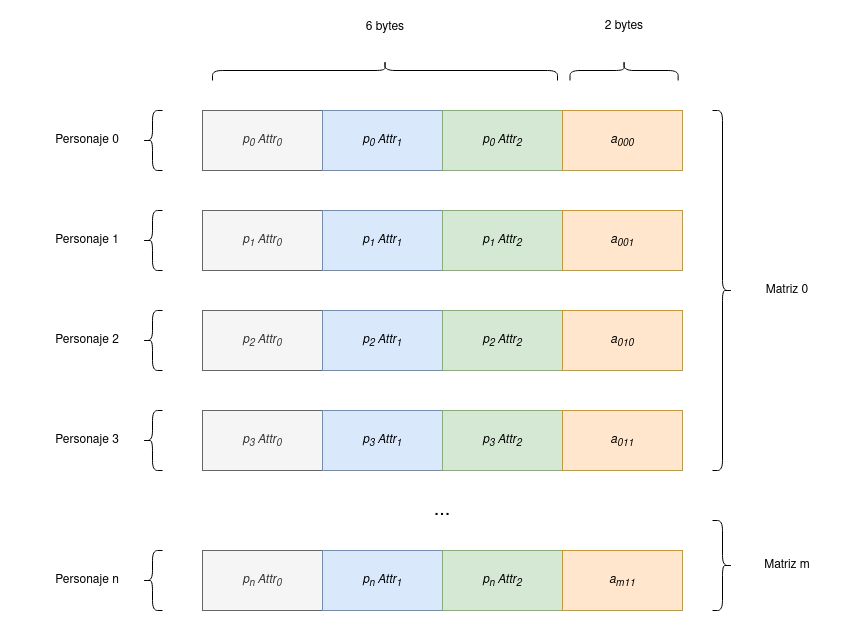
\includegraphics[height=10cm]{capitulos/capitulo3/oam_dist.png}
	\caption{Distribución de los atributos en la OAM.}
	\label{fig:oam_dist}
\end{figure}
\FloatBarrier{}

\subsubsection{Atributos}
Como se ha mencionado, las propiedades de los sprites se definen mediante tres atributos conocidos como 0, 1 y 2, que se explican a continuación. No obstante, para más información se recomienda consultar \cite{bib:gba_manual,bib:tonc}. Además, para las funciones que se puedan apreciar visualmente, se incluye un ejemplo mostrando su funcionamiento en esta sección y en la~\ref{sec:efectos}.

\vspace{1cm}
\underline{Atributo 0} \\ \\
Este atributo alberga las siguientes propiedades:

\begin{itemize}
	\item Bits \{F-E\}: Junto con los bits \{F-E\} del atributo 1, definen el tamaño de la imagen del objeto o personaje. Los tamaños posibles se pueden ver en la Tabla~\ref{tab:size}.

		\begin{table}[h]
			\centering
			\begin{tabular}{| l | l | l | l | l |}
				\hline
				\textbf{Atr. 0{\textbackslash}1} & \textbf{0} & \textbf{1} & \textbf{2} & \textbf{3}  \\ \hline
				\textbf{0} & 8x8 & 16x16 & 32x32 & 64x64  \\ \hline
				\textbf{1} & 16x8 & 32x8 & 32x16 & 64x32  \\ \hline
				\textbf{2} & 8x16 & 8x32 & 16x32 & 32x64  \\ \hline
			\end{tabular}
			\caption{Tamaño del \textit{sprite} según los valores de \{F-E\} en los atributos 0 y 1.}
			\label{tab:size}
		\end{table}
		\FloatBarrier

	\item Bit \{D\}: Bits por píxel. Este valor hay que ajustarlo dependiendo de la cantidad de colores que utilicen los \textit{tiles}. Si se iguala a 0, se utilizarán 4 bpp (bits por píxel), admitiendo una selección de 16 colores diferentes. En caso de igualarlo a 1, se utilizarán 8 bpp, ofreciendo una selección considerablemente mayor, con 256 colores diferentes. La desventaja es que cada \textit{tile} ocupará más espacio y, por lo tanto, habrá menos disponibles.
	\item Bit \{C\}: Bit de activación del efecto ``mosaico''. Este es uno de los efectos gráficos que ofrece la \textit{PPU} de la consola. Su función es ``pixelar'' todavía más el \textit{sprite} (o fondo, como se verá más adelante) en cuestión. Para utilizarlo es necesario activar este bit además de configurar el registro mostrado en la sección~\ref{sec:dispcnt}. Para más información consultar~\ref{sec:efectos_mosaico}.
	\item Bits \{B-A\}: Efectos adicionales. Están disponibles el \textit{blending} (que se consigue igualando este parámetro a 1) y el renderizado de máscara (que se consigue igualando este parámetro a 2). En caso de no especificar ningún valor (0), la \textit{PPU} renderizará el \textit{sprite} de forma normal.

		El primer modo, como su nombre sugiere, mezcla el \textit{sprite} (o fondo) con cualquier cosa que se encuentre detrás. El nivel de transparencia dependerá de los valores que se utilicen en los tres registros que usa, que se detallan posteriormente.

		El segundo no mostrará el \textit{sprite}, pero su área será utilizada para controlar cuales de los objetos o fondos que se encuentran dentro se renderizan.

	\item Bits \{9-8\}: En estos 2 bits, el programador podrá configurar cómo renderizar el \textit{sprite}. En concreto, si el objeto se rotará o cambiará de tamaño (igualando su valor a 1 o 3, respectivamente), si se ocultará (igualando a 2) o si su representación será la básica (igualando a 0), mostrando el objeto sin ningún cambio adicional. \\ \\
		Hay que resaltar que, dado que la Game Boy Advance inicializa la memoria a 0, el programador tendrá que asegurarse de que este parámetro sea 2 para todos los objetos no usados, aunque no utilice los 128 sprites disponibles. En caso contrario, en la esquina superior izquierda se mostrará el primer tile encontrado en la VRAM. Este problema se ilustra en la Figura~\ref{fig:artefacto}.

		\begin{figure}[h]
			\centering
			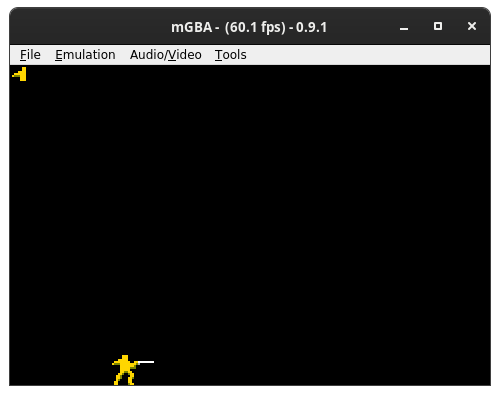
\includegraphics[width=.5\textwidth]{capitulos/capitulo3/artefacto.png}
			\caption{Resultado de no ocultar los \textit{sprites} no utilizados.}
			\label{fig:artefacto}
		\end{figure}
		\FloatBarrier

	\item Bits \{7-0\}: Las coordenadas Y del objeto siguiendo el formato especificado en la Figura~\ref{fig:y_x}.
\end{itemize}

La vista general de lo descrito anteriormente se puede observar en la Tabla~\ref{tab:sprite_attr0}. Para modificar las propiedades del atributo, el programador tiene que utilizar operadores a nivel de bit.

\begin{table}[h]
	\centering
	\begin{tabular}{| l | l |}
		\hline
		\textbf{Bits} & \textbf{Descripción} \\ \hline
		F-E & Tamaño del \textit{sprite}. \\ \hline
		D & Color utilizado. 0 para 4 bpp y 1 para 8 bpp. \\ \hline
		C & Efecto mosaico. \\ \hline
		B-A & Efectos especiales. \\ \hline
		9-8 & Modo de afinidad del objeto. \\ \hline
		7-0 & Coordenada Y del objeto. \\ \hline
	\end{tabular}
	\caption{Atributo 0.}
	\label{tab:sprite_attr0}
\end{table}
\FloatBarrier{}

\underline{Atributo 1} \\ \\
El atributo 1 incluye parámetros para invertir horizontal y verticalmente el \textit{sprite}, y otros que complementan los vistos en el atributo 0. La distribución es la mostrada a continuación:

\begin{itemize}
	\item Bits \{F-E\}: Junto con los bits \{F-E\} del atributo 0, definen el tamaño de la imagen utilizada para representar el objeto o personaje. Véase la Tabla~\ref{tab:size}.
	\item Bits \{D-C\}: Estos dos bits permiten al programador invertir tanto horizontal como verticalmente la imagen utilizada para representar el \textit{sprite}. Este recurso favorece la reutilización de los \textit{tiles} del \textit{sprite}, haciendo posible al programador invertir el objeto o personaje sin tener que guardar en memoria la imagen invertida.
		En la Figura~\ref{fig:invert_sprite} se muestra el efecto de todos los posibles valores que puede tener este campo. El primer \textit{sprite} aparece representado en su forma original, con el valor 0. El segundo \textit{sprite} se muestra invertido horizontalmente, con el valor 1. El tercer \textit{sprite} aparece invertido verticalmente, con el valor 2. Finalmente, el cuarto \textit{sprite} se representa invertido tanto horizontal como verticalmente, con el valor 3.

		\begin{figure}[h]
			\centering
			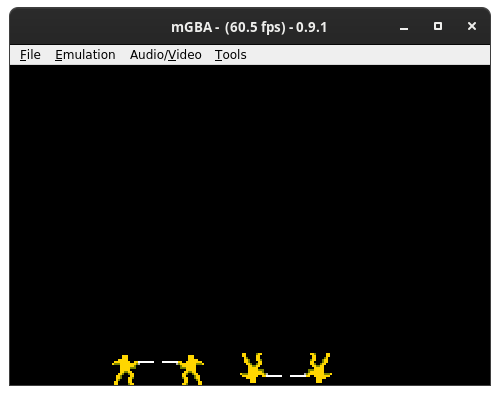
\includegraphics[width=.5\textwidth]{capitulos/capitulo3/invert_sprite.png}
			\caption{Demostración de los \textit{flags} para invertir un \textit{sprite} de diversas maneras.}
			\label{fig:invert_sprite}
		\end{figure}
		\FloatBarrier

	\item Bits \{D-9\}: En el caso de renderizar el \textit{sprite} a partir de una matriz, igualando el campo \{D-9\} del atributo 0 a 1, se especificará el índice de la matriz de afinidad a utilizar. Este valor no se podrá utilizar conjuntamente con los \textit{flags} de inversión mencionados anteriormente, dado que se superponen. No obstante, no es necesario teniendo en cuenta que se puede invertir mediante la matriz de transformación.
	\item Bits \{8-0\}: Define la coordenada X (se usará junto con la coordenada Y definida en el atributo 0).
\end{itemize}

La Tabla~\ref{tab:sprite_attr1} muestra, de manera resumida, los bits del atributo 1 junto con una breve descripción de su uso.

\begin{table}[h]
	\centering
	\begin{tabular}{| l | l |}
		\hline
		\textbf{Bits} & \textbf{Descripción} \\ \hline
		F-E & Tamaño del \textit{sprite}. \\ \hline
		D-C & \textit{Flags} para invertir el \textit{sprite}. \\ \hline
		D-9 & Índice de la matriz de transformación. \\ \hline
		8-0 & Coordenada X del objeto. \\ \hline
	\end{tabular}
	\caption{Atributo 1.}
	\label{tab:sprite_attr1}
\end{table}
\FloatBarrier{}

\underline{Atributo 2} \\ \\
El atributo 2 especifica parámetros relacionados con el renderizado de la imagen, como a partir de qué \textit{tile} se encuentra la imagen del objeto, la prioridad de renderizado y la paleta de colores a utilizar.

\begin{itemize}
	\item Bits \{F-C\}: Permiten indicar la paleta de colores a utilizar (el índice). Al igual que los \textit{flags} utilizados para invertir los \textit{sprites}, este es otro parámetro que puede ser de gran utilidad, dado que puede servir para generar personajes ``diferentes'' minimizando el uso de recursos. Un ejemplo de ello lo podemos ver en la Figura~\ref{fig:sprite_pal}.

		\begin{figure}[h]
			\centering
			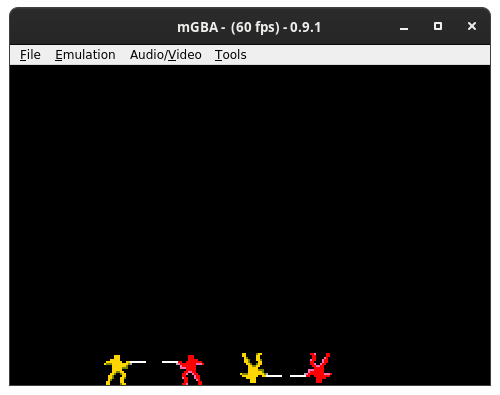
\includegraphics[width=.5\textwidth]{capitulos/capitulo3/sprite_pal.png}
			\caption{Utilizando los mismos \textit{tiles} se muestran diferentes \textit{sprites} alternando la paleta de colores de cada uno.}
			\label{fig:sprite_pal}
		\end{figure}
		\FloatBarrier

	\item Bits \{B-A\}: Este valor determina el orden con el que se renderizan los \textit{sprites} por pantalla. Cuanto mayor sea el número, antes se ``pintará'' y, por lo tanto, el objeto quedará en segundo plano al superponerse con otro de menor prioridad.
	\item Bits \{9-0\}: En estos 10 bits se especifica el primer \textit{tile} del objeto a ``pintar''. Dado que en parámetros previos se indican el tamaño de la imagen y los colores utilizados, la \textit{PPU} es capaz de saber cuántos \textit{tiles} tiene que procesar simplemente a partir del primer índice. Este valor no solo sirve para mostrar diferentes \textit{sprites} por pantalla, sino que facilita la realización las animaciones de \textit{sprites} al programador. Este solo tendría que cambiar dicho valor cada cierto tiempo.

\end{itemize}

La Tabla~\ref{tab:sprite_attr2} resume los bits utilizados, junto con una breve descripción, del atributo 2.

\begin{table}[h]
	\centering
	\begin{tabular}{| l | l |}
		\hline
		\textbf{Bits} & \textbf{Descripción} \\ \hline
		F-C & Especifica la paleta a utilizar. \\ \hline
		B-A & Prioridad de renderizado. \\ \hline
		9-0 & Índice del primer \textit{tile} del objeto. \\ \hline
	\end{tabular}
	\caption{Atributo 2.}
	\label{tab:sprite_attr2}
\end{table}


\subsubsection{Matriz de transformación}\label{sec:aff_obj}
Como se ha mencionado en los parámetros de los atributos 0 y 1, la PPU \textit{permite} al programador rotar, escalar y recortar el sprite mediante transformaciones afines. Este tipo de transformaciones, en el caso de la Game Boy Advance, se calculan con una matriz 2x2 al tratarse de un espacio 2D.

El concepto es relativamente simple. Se tiene un punto (o conjunto de puntos) definido por la ecuación \eqref{eq:eq_1} que se desea procesar. Para hacerlo, se multiplicará por la matriz de transformación, que tendrá la estructura descrita en la ecuación~\eqref{eq:eq_2}. Dependiendo de la operación que se quiera realizar, los valores $a_{00}, a_{01}, a_{10}$ y $a_{11}$ irán variando. El punto resultante, $p$, queda definido según la ecuación~\eqref{eq:eq_3}~\cite{bib:aff_matrix}:

\begin{align}
	p = 
	\begin{bmatrix}
		x\\
		y
	\end{bmatrix}
	\label{eq:eq_1}
\end{align}

\begin{align}
	A = 
	\begin{bmatrix}
		a_{00} & a_{01}\\
		a_{10} & a_{11}
	\end{bmatrix}
	\label{eq:eq_2}
\end{align}


El problema que complica ligeramente la situación al programador es que la GBA ``mapea'' los valores desde la pantalla a las texturas. Dado que el cálculo descrito en la ecuación~\eqref{eq:eq_3} es para convertir una coordenada del espacio de texturas a la pantalla, se tendrá que invertir la matriz de transformación para conseguir el resultado deseado \cite{bib:algebra}. La ecuación final quedaría como se puede observar en la ecuación~\eqref{eq:eq_4}.

\begin{align}
	p' = A  p
	\label{eq:eq_3}
\end{align}


\begin{align}
	p = A^{-1}  p'
	\label{eq:eq_4}
\end{align}

En cuanto al cálculo de la matriz inversa se refiere, al tratarse de una matriz 2x2, se puede utilizar la fórmula mostrada en~\eqref{eq:eq_5} siguiendo uno de los teoremas explicados en \cite{bib:algebra}. Aplicada a la ecuación~\eqref{eq:eq_2}, quedaría como se observa en la ecuación~\eqref{eq:eq_6}.

\begin{align}
	A^{-1} =
	\frac{1}{|A|}
	adj(A)^t
	\label{eq:eq_5}
\end{align}

\begin{align}
	\begin{bmatrix}
		a_{00} & a_{01}\\
		a_{10} & a_{11}
	\end{bmatrix}^{-1}
	=
	\frac{1}{a_{00}a_{11}-a_{01}a_{10}}
	\begin{bmatrix}
		a_{11} & -a_{01}\\
		-a_{10} & a_{00}
	\end{bmatrix}
	\label{eq:eq_6}
\end{align}

A continuación, se van a mostrar varios ejemplos junto con la matriz de transformación utilizada. Se omitirá la matriz de identidad al no modificar la imagen resultante.

Aprovechando que este recurso permite una mayor flexibilidad que los \textit{flags} de inversión del atributo 1, se probarán con ángulos que una simple inversión no puede proporcionar. El primero de ellos es un ángulo de 45º, cuya matriz, al ser de rotación, utiliza funciones coseno ($cos$) y seno ($sin$) \cite{bib:aff_matrix}. La matriz quedaría como se puede observar en la ecuación~\eqref{eq:eq_7}. Al hacer el cálculo, se obtiene que la matriz inversa es idéntica a la original.

\begin{align}
	A
	=
	A^{-1}
	=
	\begin{bmatrix}
		\cos(\theta) & -\sin(\theta)\\
		\sin(\theta) & \cos(\theta)
	\end{bmatrix}
	\label{eq:eq_7}
\end{align}
\newpage
La Figura~\ref{fig:rot_45} incluye el resultado de usar esta matriz con los ejemplos anteriores.

\begin{figure}[h]
	\centering
	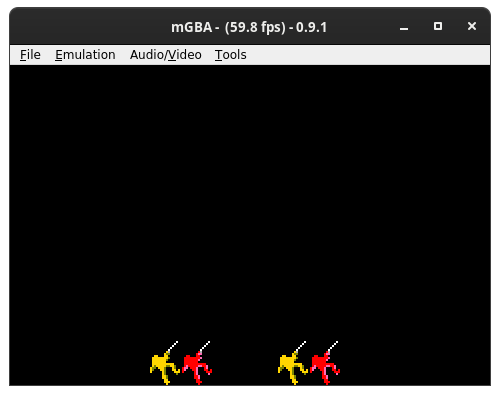
\includegraphics[width=.5\textwidth]{capitulos/capitulo3/rot_45.png}
	\caption{Rotación de \textit{sprites} por medio de la matriz de transformación.}
	\label{fig:rot_45}
\end{figure}
\FloatBarrier

Otra matriz utilizada a menudo es la de escalado. Como su nombre indica, permite aumentar el tamaño del \textit{sprite} tanto en el eje X como en el Y \cite{bib:aff_matrix}. La matriz utilizada en este ejemplo se muestra en la ecuación \eqref{eq:eq_7}, siendo $a$ el factor de escalado en el eje X y $d$ el factor de escalado en Y. La inversa quedaría como se muestra en la ecuación~\eqref{eq:eq_9}.

\begin{align}
	A
	=
	\begin{bmatrix}
		a & 0 \\
		0 & d
	\end{bmatrix}
	\qquad
\end{align}

\begin{align}
	A^{-1}
	=
	\begin{bmatrix}
		1/a & 0 \\
		0 & 1/d
	\end{bmatrix}
	\label{eq:eq_9}
\end{align}

El resultado de multiplicar por 2 tanto el eje X como Y en el programa de demostración es el que se muestra en la Figura~\ref{fig:scale_2}.

\begin{figure}[h]
	\centering
	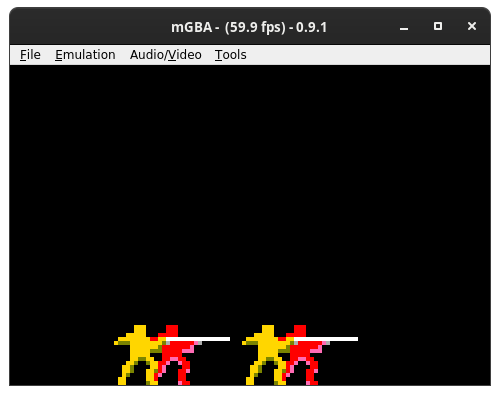
\includegraphics[width=.5\textwidth]{capitulos/capitulo3/scale_2.png}
	\caption{Escalado \textit{sprites} por medio de una matriz de transformación.}
	\label{fig:scale_2}
\end{figure}
\FloatBarrier{}

En caso de querer rotar y escalar el \textit{sprite} a la vez, esto se puede realizar combinando las fórmulas mostradas anteriormente (ecuaciones~\eqref{eq:eq_10} y~\eqref{eq:eq_11}), tal y como se muestra en la ecuación \eqref{eq:eq_12}.

\begin{align}
	A_e^{-1}
	=
	\begin{bmatrix}
		1/a & 0 \\
		0 & 1/d
	\end{bmatrix}
	\label{eq:eq_10}
\end{align}

\begin{align}
	A_r^{-1}
	=
	\begin{bmatrix}
		\cos(\theta) & -\sin(\theta)\\
		\sin(\theta) & \cos(\theta)
	\end{bmatrix}
	\label{eq:eq_11}
\end{align}

\begin{align}
	A_{re}^{-1}
	=
	\begin{bmatrix}
		1/a & 0 \\
		0 & 1/d
	\end{bmatrix}
	\begin{bmatrix}
		\cos(\theta) & -\sin(\theta)\\
		\sin(\theta) & \cos(\theta)
	\end{bmatrix}
	=
	\begin{bmatrix}
		\cos(\theta)/a & -\sin(\theta)/a\\
		\sin(\theta)/d & \cos(\theta)/d
	\end{bmatrix}
	\label{eq:eq_12}
\end{align}

Esto da lugar a la Figura~\ref{fig:scale_and_rot}, en la que se combina una rotación de 30º con un factor de escala de 1.5 en los dos ejes.

\begin{figure}[h]
	\centering
	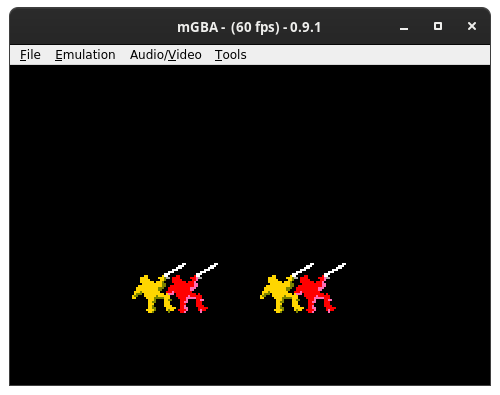
\includegraphics[width=.55\textwidth]{capitulos/capitulo3/rot_scale_30_1.5.png}
	\caption{Rotación y escalado de \textit{sprites} por medio de la matriz de transformación.}
	\label{fig:scale_and_rot}
\end{figure}
\FloatBarrier{}

Lamentablemente, este sistema trae consigo varias limitaciones y problemas. El primero de ellos es la imposibilidad de rotar, escalar y realizar transformaciones de corte si el \textit{sprite} resultante sobrepasa el área original establecida (el tamaño original del \textit{sprite}, véase la Tabla~\ref{tab:size}). Esto se puede resolver igualando el parámetro \{9-8\} del atributo 0 a 3, duplicando el área original del objeto. Sin embargo, si el \textit{sprite} sobrepasa esa área, también se verá cortado (véase la Figura~\ref{fig:too_big}). Además, el programador deberá tener en cuenta el cambio en las coordenadas X e Y al posicionar el \textit{sprite} en pantalla.


\begin{figure}[h]
	\centering
	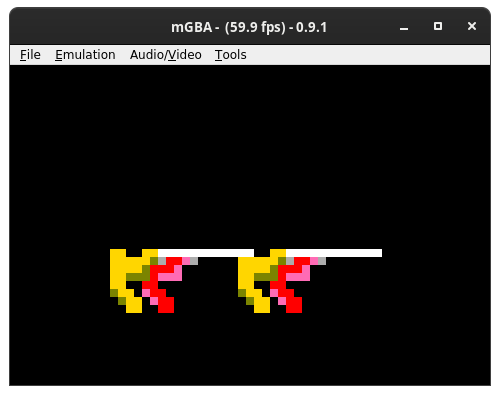
\includegraphics[width=.55\textwidth]{capitulos/capitulo3/too_big.png}
	\caption{\textit{Sprite} que sobrepasa el área permitida.}
	\label{fig:too_big}
\end{figure}
\FloatBarrier{}

La segunda limitación es el uso, en varios casos, de operaciones en punto flotante y funciones $cos$ y $sin$. El hecho de que la consola no cuente con una \textit{FPU} (\textit{Floating Point Unit}) ralentiza de manera considerable el cálculo. Por lo tanto, habrá que evitar este tipo de operaciones no solo al calcular la matriz de transformación, sino en otros aspectos del programa también. De hecho, el dispositivo no acepta \textit{floats} como valores de la matriz de transformación, solo permite números de coma fija (\textit{fixed point numbers} en inglés). El uso de este tipo de números se verá con más detenimiento en la Sección~\ref{sec:aspectos}.

\subsection{Bitmaps}\label{sec:bitmaps}
A diferencia de sus predecesoras, la Game Boy Advance proporciona al programador una forma directa de manipular los píxeles que aparecen por pantalla, lo que se conoce como \textit{bitmap}. Este modo, considerado como el más simple de los que ofrece el dispositivo, trata el contenido de la sección de memoria VRAM como los píxeles de la pantalla. Por lo tanto, con escribir en esta dirección de memoria, la pantalla inmediatamente representará los cambios reflejados sin tener que cambiar o configurar ningún registro o atributo adicional.

Este modo no es del todo práctico ni eficiente, dado que se tiene que suministrar el valor de cada uno de los píxeles que aparecen por pantalla. Sin embargo, sigue siendo válido para mostrar imágenes estáticas, realizar juegos relativamente simples (como \textit{Pong}) o 3D como \textit{Doom}\footnote{\url{https://doom.fandom.com/wiki/Game_Boy_Advance}}.

Concretamente, existen tres modos \textit{bitmap} para manipular directamente los píxeles. Se diferencian en aspectos como el tamaño del \textit{canvas}, si se recurre a una paleta de colores o si se cuenta con un buffer adicional  \cite{bib:gba_manual}.

La Tabla~\ref{tab:modos_bitmap} resume las diferencias principales de los modos, de los que se dan más detalles en las siguientes subsecciones.

\begin{table}[h]
	\centering
	\begin{tabular}{| l | l | l | l | l | l |}
		\hline
		\textbf{Modo} & \textbf{Ancho} & \textbf{Alto} & \textbf{bpp} & \textbf{Uso de paleta} & \textbf{Buffer adicional} \\ \hline
		3 & 240 & 160 & 16 & No & No \\ \hline
		4 & 240 & 160 & 8 & Sí & Sí \\ \hline
		5 & 160 & 128 & 16 & No & Sí \\ \hline
	\end{tabular}
	\caption{Modos bitmap de la Game Boy Advance. Tabla basada en \cite{bib:tonc}}
	\label{tab:modos_bitmap}
\end{table}
\FloatBarrier{}

\subsubsection{Modo 3}\label{sec:mode_3}
El modo 3 ofrece al programador un buffer de 240x160 de 16 bits por píxel, resolución que coincide con la pantalla de la Game Boy Advance. De los 16 bits, se utilizan 15 para cada color como se mostró en la Tabla~\ref{tab:15bit_color}. En total, este buffer ocupa 75 KB, desde la dirección 0x06000000 (VRAM) \cite{bib:gba_manual}.

\begin{figure}[h]
	\centering
	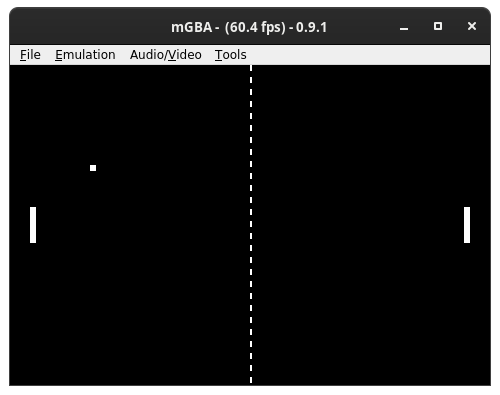
\includegraphics[width=.55\textwidth]{capitulos/capitulo3/bitmaps_3.png}
	\caption{Demostración práctica del uso del Modo 3.}
	\label{fig:modo_3}
\end{figure}
\FloatBarrier

En la Figura~\ref{fig:modo_3} se puede observar un ejemplo de un juego simple que utiliza el modo 3 de la \textit{PPU}.

Como dato adicional, es posible utilizar conjuntamente los modos \textit{bitmaps} y el modo de \textit{sprites}. Sin embargo, en el caso del modo 3 se disminuye el espacio destinado a \textit{tiles} un 50\% \cite{bib:tonc}.

\subsubsection{Modo 4}\label{sec:mode_4}
El modo 4, a pesar de utilizar un \textit{canvas} idéntico al modo 3, de 240x160 también, incluye varias opciones interesantes para el programador.

Para empezar, en lugar de guardar los valores de los píxeles directamente en la VRAM, guarda los índices de la paleta de colores que se encuentra en la RAM de paleta. A la hora de modificar el color de una gran cantidad de píxeles, esto puede suponer una ventaja en términos de rendimiento con respecto al modo 3. Dada la inherente ineficiencia que supone modificar cada uno de los píxeles que aparecen por pantalla, tener índices apuntando a una paleta de colores permite al programador cambiar un gran número de píxeles simplemente cambiando uno de los valores de la paleta.

Además, al utilizar índices, que ocupan 8 bits, el espacio dedicado a la imagen se reduce a la mitad. Este espacio ``extra'' lo aprovecha un buffer que ofrece el modo 4. Este buffer adicional se encuentra en la dirección de memoria 0x0600A000. El buffer principal del modo 4 acaba en 0x06009600, por lo que no interfiere con el segundo buffer disponible. La idea es que el programador escriba el próximo ``frame'' en el buffer no activo para posteriormente modificar el buffer activo. Así se consigue que los cambios realizados no hagan que la imagen final sufra \textit{tearing}, es decir, que no se superpongan imágenes de forma indebida~\cite{bib:gba_manual,bib:tonc}.

\subsubsection{Modo 5}\label{sec:mode_5}
El modo 5 ofrece tanto la posibilidad de escribir directamente en VRAM sin tener que utilizar una paleta con color de 15 bits, como un segundo buffer donde preparar el siguiente frame. Aunque, en detrimento del jugador, usa un canvas de dimensiones reducidas, de 160x128 \cite{bib:gba_manual}. La Figura~\ref{fig:modo_5} da una idea al lector del área que abarca este modo.

\begin{figure}[h]
	\centering
	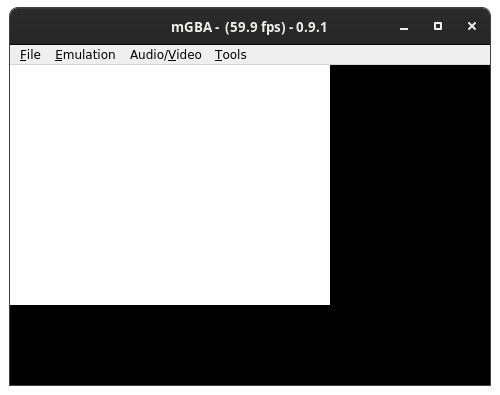
\includegraphics[width=.55\textwidth]{capitulos/capitulo3/bitmaps_5.png}
	\caption{Ejemplo práctico del modo 5.}
	\label{fig:modo_5}
\end{figure}
\FloatBarrier

Al igual que el modo 3, el modo 5 usa gran parte de la VRAM, lo que reduce el número de \textit{tiles} disponibles para \textit{sprites} \cite{bib:tonc}.

\subsection{Fondos}\label{sec:fondos}
Los fondos de la GBA permiten especificar mediante el uso de ``mapas'' qué \textit{tiles} utilizar para rellenar el canvas. A pesar de que técnicamente los \textit{bitmaps} se catalogan como fondos en el manual \cite{bib:gba_manual}, se suelen separar los modos 0, 1, 2 y 3 de los modos 4, 5 y 6 por las grandes diferencias de funcionamiento.

A diferencia de los \textit{sprites}, la mayor parte de la configuración se hace en los registros de configuración específicos para los fondos. Por lo tanto, lo que hay que tener en cuenta al mostrar fondos en la consola es el formato que sigue cada una de las entradas del mapa, que especifica el \textit{tile} a utilizar y el número y tipo de fondos a emplear.

En cuanto al formato que sigue una entrada del mapa correspondiente a un fondo, tiene la siguiente distribución:

\begin{itemize}
	\item Bits \{F-C\}: Índice de la paleta de colores a utilizar en caso de estar en el modo de color de 4 bpp.
	\item Bits \{B-A\}: Es similar a lo visto en el atributo 1 de los \textit{sprites}. Permite invertir tanto horizontal como verticalmente el \textit{tile} especificado en los bits \{9-0\}.
	\item Bits \{9-0\}: Índice del \textit{tile} a utilizar.
\end{itemize}

Sin embargo, con las herramientas disponibles, el programador no tendrá que preocuparse del formato que sigue cada entrada en el mapa. Las utilidades como Grit ya automatizan la generación de los mapas de cada fondo.

Lo que si tiene que tener en cuenta el programador son los modos que configurará en los registros mostrados en la sección~\ref{sec:conf_fondos}, indicando cuántos de los 4 fondos disponibles planea utilizar y si utilizarán una matriz de transformación. Dependiendo de los modos seleccionados, unos fondos u otros quedarán inhabilitados o limitados a un uso específico. En la Tabla~\ref{tab:modos_fondos} se denota con ``r'' a los fondos normales y con ``t'' a los fondos que utilizan la matriz de transformación.

\begin{table}[h]
	\centering
	\begin{tabular}{| l | l | l | l | l |}
		\hline
		\textbf{Modo} & \textbf{Fondo 0} & \textbf{Fondo 1} & \textbf{Fondo 2} & \textbf{Fondo 3} \\ \hline
		0 & r & r & r & r \\ \hline
		1 & r & r & t  & - \\ \hline
		2 & - & - & t & t \\ \hline
	\end{tabular}
	\caption{Modos para los fondos de la Game Boy Advance.}
	\label{tab:modos_fondos}
\end{table}

Otro aspecto que se ve afectado por el modo seleccionado es el tamaño del fondo. Tal y como se puede observar en la Tabla~\ref{tab:size_bg}, el tamaño del fondo depende en parte de si utiliza una matriz de transformación. El valor de la columna \textit{flag} es el que le corresponde a los bits \{F-E\} en el registro de control. Los valores mostrados utilizan como base el \textit{tile} de 8x8 y, para dar una mejor idea del tamaño, se incluye entre paréntesis el tamaño en píxeles del fondo.

\begin{table}[h]
	\centering
	\begin{tabular}{| l | l | l |}
		\hline
		\textbf{Flag} & \textbf{Tamaño para \textit{r}} & \textbf{Tamaño para \textit{t}} \\ \hline
		00 & 32x32 (256x256) & 16x16 (128x128) \\ \hline
		01 & 64x32 (512x256) & 32x32 (256x256) \\ \hline
		10 & 32x64 (256x512) & 64x64 (512x512) \\ \hline
		11 & 64x64 (512x512) & 128x128 (1024x1024) \\ \hline
	\end{tabular}
	\caption{Tamaños disponibles para cada uno de los fondos.}
	\label{tab:size_bg}
\end{table}
\FloatBarrier{}

Una demostración de un fondo renderizado se puede observar en la Figura~\ref{fig:fondo_1}. Se trata de un fondo de 32x32 (o 256x256 píxeles) en movimiento actualizando los valores de los registros de offset.

\begin{figure}[h]
     \centering
         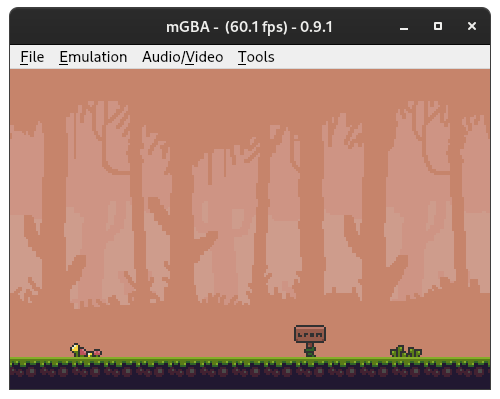
\includegraphics[width=.55\textwidth]{capitulos/capitulo3/fondo_1.png}
	\caption{Fondo 32x32.}\label{fig:fondo_1}
\end{figure}
\FloatBarrier{}

Además de las diferencias de tamaño observadas en la Tabla~\ref{tab:size_bg}, los fondos que utilizan la matriz de transformación también ven las entradas del mapa modificadas. En este caso se prescinde del índice de paleta y de la orientación de cada \textit{tile}. De esta forma, cada entrada del mapa acaba siendo solo el índice del mapa y su tamaño se ve reducido a 1 byte \cite{bib:tonc}.

Basándose en los mismos conceptos vistos en la sección~\ref{sec:aff_obj}, hay que definir los valores de una matriz 2x2 para modificar el fondo en cuestión. En la Figura~\ref{fig:fondos_aff} se ofrecen dos variantes del fondo mostrado en la Figura~\ref{fig:fondo_2} cambiando el tamaño y la rotación del mismo.

\begin{figure}[h]
     \centering
         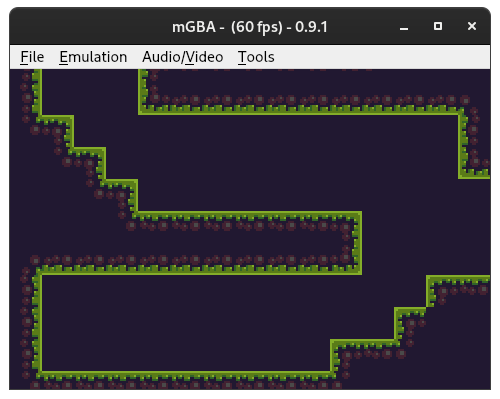
\includegraphics[width=.55\textwidth]{capitulos/capitulo3/affine_bg_1.png}
	\caption{Fondo 32x32.}\label{fig:fondo_2}
\end{figure}
\FloatBarrier{}

\begin{figure}[h]
     \centering
     \begin{subfigure}[b]{0.45\textwidth}
         \centering
         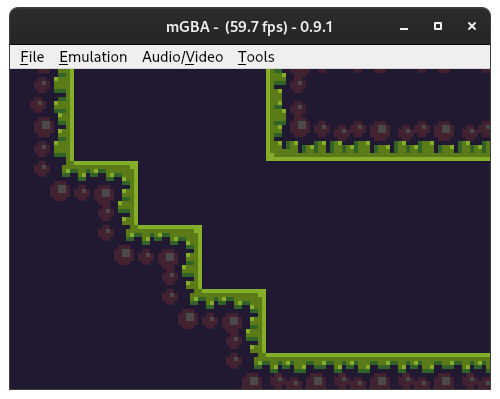
\includegraphics[width=\textwidth]{capitulos/capitulo3/affine_bg_2.png}
         \label{fig:fondo_3}
	     \caption{Fondo escalado un 100\%.}
     \end{subfigure}
     \hfill
     \begin{subfigure}[b]{0.45\textwidth}
         \centering
         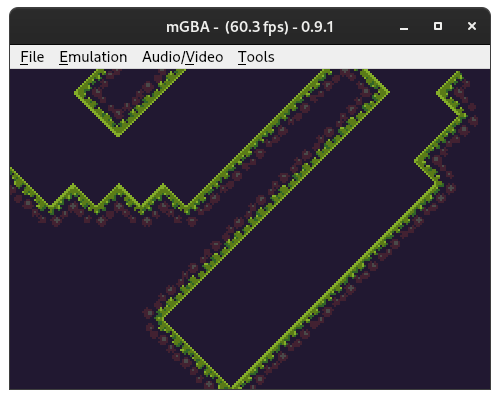
\includegraphics[width=\textwidth]{capitulos/capitulo3/affine_bg_3.png}
         \label{fig:fondo_4}
	     \caption{Fondo rotado por 45º.}
     \end{subfigure}
	\caption{Matriz de transformación sobre el fondo de la Figura~\ref{fig:fondo_2}.}\label{fig:fondos_aff}
\end{figure}
\FloatBarrier{}

\subsection{Efectos especiales}\label{sec:efectos}
La GBA ofrece al programador diversas formas de pulir y refinar sus juegos con efectos especiales acelerados por hardware. Los cuatro efectos especiales son el \textbf{\textit{blending}}, \textbf{efectos \textit{fade in/out}}, el \textbf{modo ``mosaico''} y el \textbf{modo ventana}.

Todos ellos se pueden aplicar tanto a \textit{sprites} como a fondos. El efecto no varía si se aplica a un objeto o a un fondo, por lo que los ejemplos mostrados valen para ambos.

\subsubsection{\textit{Blending}}\label{sec:efectos_blending}
Como su nombre sugiere, permite mezclar los colores que se encuentran detrás del \textit{sprite}, ya sea un fondo u otro \textit{sprite}. El nivel del efecto se configura en los registros adicionales vistos en el sección~\ref{sec:dispcnt}.

El registro que guarda los coeficientes de mezcla, BLDALPHA (para más información consultar el sección~\ref{sec:dispcnt}), calcula el valor de cada píxel siguiendo la fórmula mostrada en la ecuación~\eqref{eq:blending}. El cálculo se realiza para cada color de forma separada, de ahí el mínimo de 31, número que representa el máximo valor que puede alcanzar un color de 5 bits.

\begin{align}
	valor
	=
	min(31, color_{frontal} * coef_{frontal} + color_{posterior} * coef_{posterior})	
	\label{eq:blending}
\end{align}

Una demostración del efecto que se consigue con el \textit{sprite} utilizado anteriormente combinado con un fondo gris se puede observar en la Figura~\ref{fig:blending}.

\begin{figure}[h]
     \centering
     \begin{subfigure}[b]{0.45\textwidth}
         \centering
         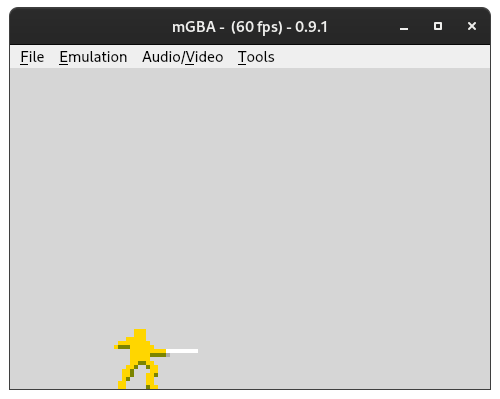
\includegraphics[width=\textwidth]{capitulos/capitulo3/blending_1.png}
         \label{fig:blending_1}
	     \caption{Demostración sin \textit{blending}.}
     \end{subfigure}
     \hfill
     \begin{subfigure}[b]{0.45\textwidth}
         \centering
         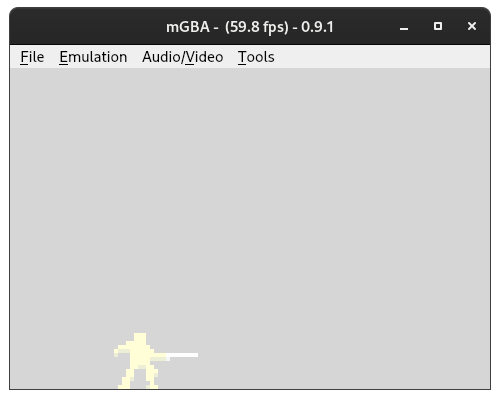
\includegraphics[width=\textwidth]{capitulos/capitulo3/blending_2.png}
         \label{fig:blending_2}
	     \caption{Demostración con \textit{blending}.}
     \end{subfigure}
	\caption{Efecto conseguido configurando el efecto \textit{blending} de la consola.}\label{fig:blending}
\end{figure}
\FloatBarrier{}

\subsubsection{Efectos \textit{fade}}\label{sec:efectos_fade}
Para facilitar las transiciones entre escenas, la \textit{PPU} ofrece la posibilidad de cambiar gradualmente de una imagen a otra completamente negra, y de una imagen a otra completamente blanca. 

Configurando los registros BLDCNT y BLDY vistos en la sección~\ref{sec:dispcnt}, se modifica la intensidad de la imagen mostrada por pantalla. Si se actualiza el valor de BLDY se conseguirá el deseado efecto \textit{fade in/out}. En las Figura~\ref{fig:brightness} se muestra un aumento y disminución de la intensidad sobre una imagen. 

\begin{figure}[h]
     \centering
     \begin{subfigure}[b]{0.45\textwidth}
         \centering
         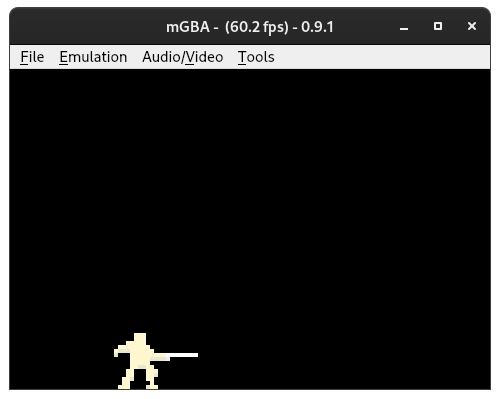
\includegraphics[width=\textwidth]{capitulos/capitulo3/brightness_3.png}
         \label{fig:blending_1}
	     \caption{Aumento de la intensidad.}
     \end{subfigure}
     \hfill
     \begin{subfigure}[b]{0.45\textwidth}
         \centering
         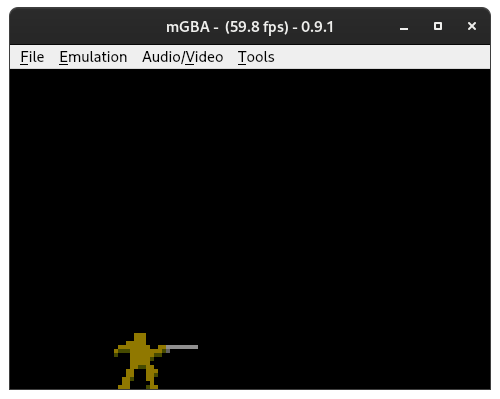
\includegraphics[width=\textwidth]{capitulos/capitulo3/brightness_4.png}
         \label{fig:blending_2}
	     \caption{Disminución de la intensidad.}
     \end{subfigure}
	\caption{Demostración del cambio de intensidad a través de BLDCNT y BLDY.}\label{fig:brightness}
\end{figure}
\FloatBarrier{}

\subsubsection{Modo mosaico}\label{sec:efectos_mosaico}
Este modo reduce el nivel de detalle de un objeto o fondo. Para ello, la GBA internamente aplica el valor de un píxel a los vecinos posicionados debajo y a su derecha. El número de píxeles que acaban compartiendo el mismo valor quedará determinado por el número de distorsión horizontal y vertical que se indique en el registro correspondiente. Por ejemplo, si el píxel 0 tiene un valor determinado y la distorsión horizontal es de 10, entonces los píxeles 1-10 tendrán el mismo color que el píxel 0. Siguiendo el ejemplo, si la distorsión horizontal es de 10, el siguiente píxel a tener en cuenta sería el 11.
Un ejemplo del efecto se puede observar en la Figura~\ref{fig:mosaic}.

		\begin{figure}[h]
			\centering
			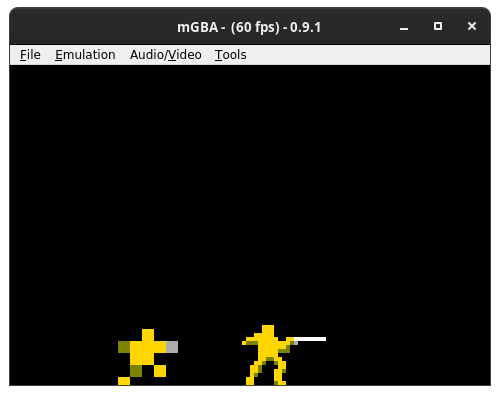
\includegraphics[width=.45\textwidth]{capitulos/capitulo3/mosaic.png}
			\caption{Sprite renderizado con efecto ``mosaico'' (izquierda), junto a su representación sin alterar (derecha).}
			\label{fig:mosaic}
		\end{figure}
		\FloatBarrier


\subsubsection{Modo ventana}\label{sec:efectos_ventana}
El último efecto destacable que ofrece la GBA es la posibilidad de crear ventanas en pantalla y controlar qué contenido es renderizado dentro y fuera de ellas. La consola proporciona 2 ventanas para fondos, y cada \textit{sprite} puede configurarse para controlar qué se renderiza dentro y fuera del área que ocupa. En caso de superponerse las dos ventanas disponibles, el contenido renderizado es la unión del contenido permitido en ambas. Por otra parte, el contenido no renderizado es todo lo que no entra en la unión mencionada anteriormente.

La Figura~\ref{fig:windows} muestra un ejemplo sobre el fondo de la Figura~\ref{fig:fondo_1}. En este ejemplo se observa una ventana que ocupa la mitad de la pantalla en la que se permite el renderizado de dos fondos (el fondo con el paisaje y el fondo con la vegetación). Fuera de la ventana, solo se permite el renderizado de uno de los fondos (el de la vegetación).

\begin{figure}[b]
	\centering
	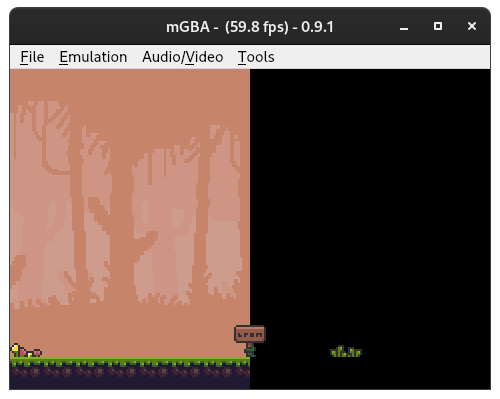
\includegraphics[width=.45\textwidth]{capitulos/capitulo3/window_1.png}
	\caption{Demostración del funcionamiento de una ventana.}
	\label{fig:windows}
\end{figure}
